\documentclass[a4paper]{report}
\usepackage{a4wide}
%\documentclass{scrreprt}

% Circumvent KOMA Script' strict 1:2 top margin to bottom margin relation
%\usepackage[hscale=0.71,vscale=0.8,vmarginratio={6:8},heightrounded]{geometry}

\usepackage[utf8]{inputenc}   % Literal typing of ä, ö, ü
\usepackage{amssymb,amsmath}
\usepackage{hyperref}
\usepackage{array}            % For \newcolumntype
\usepackage{tikz}
\usepackage{tikz-qtree}

\usetikzlibrary{
  shapes,
  arrows,
  positioning,  % Function "of" (e.g. [right=of x])
  automata,     % Styles "state", "initial", "accepting"
  backgrounds,  % Predefined layer named "background"
  calc          % Calculations $...$
}

\newcommand{\om}{{$\omega$}}
\newcommand{\x}[1]{\widehat{#1}}               % Colour -1
\newcommand{\one}[1]{\overline{#1}}            % Colour  1
\newcommand{\two}[1]{\overline{\overline{#1}}} % Colour  2

% Table column: fixed width, horizontally, vertically centered
\newcolumntype{C}[1]{>{\centering\let\newline\\\arraybackslash\hspace{0pt}}m{#1}}

% Table spacings
{\renewcommand{\arraystretch}{1.15}
\renewcommand{\tabcolsep}{0.1cm}  

% Indentation of second and following lines figure captions. Default indentation
% in KOMA script is length of "Figure X.X: ".
% \setcapindent{2em}

% Used as "TikZ variables"
\def\myvdist{1.2cm}  % Level distance of tree
\def\myhdist{0.5cm}  % Sibling distance of tree
\def\myndist{1cm}    % Node distance for automata

% Math strings
\newcommand{\q}  [1]{$q_{#1}$}            % \q0    --> $q_0$
\newcommand{\qq} [1]{$\{q_{#1}\}$}        % \qq0   --> ${q_0}$
\newcommand{\qqq}[2]{$\{q_{#1},q_{#2}\}$} % \qqq01 --> ${q_0,q_1}$
\newcommand{\qm} [1]{\{q_{#1}\}}          % \qm0   --> {q_0}

\tikzset{
  font=\scriptsize\sffamily,
  semithick,
  >=stealth,
  longer1/.style={
    shorten >=-0.425mm,
    shorten <=-0.5mm
  },
  longer2/.style={
    shorten >=-0.7mm,
    shorten <=-0.8mm
  },
  my state/.style={
    draw,
    minimum height=1.75em,
    minimum width=2em,
    inner sep=1mm,
    rectangle,
    rounded corners=2mm
  },
  my accepting/.style={
    double,
    double distance=1pt,
    outer sep=0.9pt,
    semithick
  },
  automaton/.style={
    every state/.style={my state},
    accepting/.style={my accepting},
    initial text=,
    every loop/.style={min distance=6mm,looseness=7},
    my below/.style={out=295,in=245},
    my above/.style={out=65,in=115},
    node distance=\myndist
  },
  tree/.style={
    s/.style={my state},
    a/.style={my state,my accepting},
    level distance=\myvdist,
    sibling distance=\myhdist,
  },
  tree example sets/.style={
    0/.style= {st,font={$\{q_0\}$}},
    1/.style= {st,acc,font={$\{q_1\}$}},
    2/.style= {st,font={$\{q_2\}$}},
    02/.style={st,font={$\{q_0,q_2\}$}},
  },
  tree example no sets/.style={
    0/.style={st,font={$q_0$}},
    1/.style={st,acc,font={$q_1$}},
    2/.style={st,font={$q_2$}},
  },
  dag/.style={
    s/.style={my state},
    a/.style={my state,my accepting},
    row sep={\myvdist,between origins},
    column sep=0.75cm,
    inner sep=0mm,
    ghost/.style={draw=black!20,color=black!20},
  }
}

\newcommand{\automaton}{
\begin{tikzpicture}[automaton]
\node[state,initial]   (0)                    {\q0};
\node[state,accepting] (1) [above right=of 0] {\q1};
\node[state]           (2) [below right=of 1] {\q2};
\path[->] (0) edge[my below,loop] node[below]           {$a$} ()
              edge[longer1]       node[pos=0.3,above](m){$a$} (1)
              edge                node[below]           {$a$} (2)
          (1) edge[longer1]       node[pos=0.7,above]   {$a$} (2)
          (2) edge[my below,loop] node[below]           {$a$} ();
\node[draw=none,anchor=base,xshift=-1.5cm] at (m.base){$A=$};  
\end{tikzpicture}
}

\newcommand{\symbols}{
\begin{tikzpicture}[tree,l/.style={pos=0.3,font={$a$}},e/.style={draw=none}]
\Tree [ \edge[e] node[l]{}; [ \edge[e] node[l]{}; [ \edge[e] node[l]{}; [ \edge[e] node[l]{}; {} ] ] ] ]
\end{tikzpicture}
}

\begin{document}
% Title page
\title{Performance Investigation of a Subset-Tuple Büchi Complementation Construction}
\author{Daniel Weibel}
\date{\today}
\maketitle

% Abstract
% \begin{abstract}
% Hello world
% \end{abstract}

% Table of contents
\tableofcontents

\chapter{Introduction}
At the beginning of the 1960s, a Swiss logician named Julius Richard Büchi at Michigan University was looking for a way to prove the decidability of the satisfiability of monadic second order logic with one successor (S1S). Büchi applied a trick that truly founded a new paradigm in the application of logic to theoretical computer science. He thought of interpretations of a S1S formula as infinitly long words of a formal language and designed a type of finite state automaton that accepts such a word if and only if the interpretation it represents satisfies the formula. After proving that every S1S formula can be translated to such an automaton and vice versa (Büchi's Theorem), the satisfiabilty problem of an S1S formula could be reduced to testing the non-emptiness of the corresponding automaton.

This special type of finite state automaton was later called Büchi automaton.

% Context of study
A Büchi complementation construction takes as input a Büchi automaton $A$ and produces as output another Büchi automaton $B$ which accepts the complement language of the input automaton $A$. Complement language denotes the ``contrary'' language, that is, $B$ must \emph{accept} (over a given alphabet) every word that $A$ \emph{does not} accept, and must in turn \emph{not accept} every word that $A$ \emph{accepts}.

Büchi automata are finite automata (that is, having a finite number of states) which operate on infinite words (that is, words that ``never end''). Operating on infinite words, they belong thus to the category \om-automata. An important application of Büchi automata is in model checking which is a formal system verification technique. There, they are used to represent both, the description of the system to be checked for the presence of a correctness property, and (the negation of) this correctness property itself.

In one approach to model checking, the correctness property is directly specified as a Büchi automaton
One approach to model checking requires that the Büchi automaton representing the correctness property is complemented. It is here that the problem of Büchi complementation has one of its practical applications. 

% Stating the problem, reason the research is worth tackling
The complementation of non-deterministic Büchi automata is hard. It has been proven to have an exponential lower bound in the number of generated states [cite]. That is, the number of states of the output automaton is, in the worst case, an exponential function of the number of states of the input automaton. However, since the introduction of Büchi automata in the 1960's, significant process in reducing the complexity (in other words, the degree of exponentiality) of the Büchi complementation problem has been made. Some numbers [list complexities of the different constructions].

% Aim and scope

% Significance: advance knowledge, contribute to solutin of practical problem, novel use of a procedure or technique?

% Overview


% 2. The Büchi complementation problem
% 2.1 Preliminaries
% Used naming convention (NBW, DBW, etc.)
%   2.1.1 Büchi automata
%     - Definition
%     - DBW vs. NBW
%     - Equivalence with omega-regular languages (NBW)
%     - DBW weaker than NBW (proof)
%   2.1.2 Other omega-automata
%     - Muller, Rabin, Streett, Parity
%     - McNaughton's Theorem (NBW = DMW)
%     - Complete picture of equivalences
%   2.1.3 Complementation of Büchi automata
%     - NBW closed under complementation (DBW not, proof)
%     - Example NFA/DFA
%     - Complementation of DBW (Kurshan)
%   2.1.4 Complexity of Büchi Complementation
%     - Notion of state blow-up
%     - Lower bounds for the state blow-up
% 2.2 Review of Büchi Complementation Constructions
% 2.3 Empirical Performance Investigations
\chapter{The Büchi Complementation Problem}
\section{Preliminaries}
\subsection{Büchi Automata}
Büchi automata have been introduced in 1962 by Büchi~\cite{buchi1960decision} in order to show the decidability of monadic second order logic; over the successor structure of the natural numbers~\cite{2012_breuers}.

he had proved the decidability of the monadic-second order theory of the natural numbers with successor func- tion by translating formulas into finite automata~\cite{vardi2007automata} (p. 1)

%To check whether a given S1S formulaφ=φ(V0,...,Vm−1)is satisfiable one simply constructs the Büchi automaton which is guaranteed to exist by Büchi’s Theorem and checks this automaton for non-emptiness~\cite{vardi2007automata} (p. 9).

Büchi needed to create a complementation construction (proof the closure under complementation of Büchi automata) in order to prove Büchi's Theorem.

Büchi's Theorem: S1S formulas and Büchi automata are expressively equivalent (there is a NBW for every S1S formula, and there is a S1S formula for every NBW).

\subsubsection{Definitions}
Informally speaking, a Büchi automaton is a finite state automaton running on input words of infinite length. That is, once started reading a word, a Büchi automaton never stops. A word is accepted if it results in a run (sequence of states) of the Büchi automaton that includes infinitely many occurrences of at least one accepting state.
% A word is accepted by a Büchi automaton, if there exists a run (sequence of states) for it that includes infinite repetitions of at least one accepting state. In other words, if during reading a word a Büchi automaton goes through one or more accepting states infinitely often, the word is accepted, and otherwise it is rejected.

More formally, a Büchi automaton $A$ is defined by the 5-tuple $A = (Q, \Sigma, q_0, \delta, F)$ with the following components.
\begin{itemize}
\item $Q$: a finite set of states
\item $\Sigma$: a finite alphabet
\item $q_0$: an initial state, $q_0 \in Q$
\item $\delta$: a transition function, $\delta: Q \times \Sigma \rightarrow 2^Q$ %(mapping combinations of a state and a symbol to zero, one, or more other states)
\item $F$: a set of accepting states, $F \in 2^Q$
\end{itemize}

We denote by $\Sigma^\omega$ the set of all words of infinite length over the alphabet $\Sigma$. A Büchi automaton runs on the elements of $\Sigma^\omega$. In the following, we define the acceptance behaviour of a Büchi automaton $A$ on a word $\alpha \in \Sigma^\omega$.

% A Büchi automaton runs on infinite words over the alphabet $\Sigma$. We denote by $\Sigma^\omega$ the set of all possible words of infinite length (\om-words) over $\Sigma$. 

% What distinguishes a Büchi automaton from a finite state automaton on finite words are its conditions for accepting or rejecting words. In the following, we define the acceptance behaviour of a Büchi automaton.

\begin{itemize}
% \item $\Sigma^\omega$ is the set of all possible words of infinite length over alphabet $\Sigma$
\item A \emph{run} of Büchi automaton $A$ on a word $\alpha \in \Sigma^\omega$ is a sequence of states $q_0q_1q_2\dots$ such that $q_0$ is $A$'s initial state and $\forall i \geq 0: q_{i+1} \in \delta(q_i, \alpha_i)$
\item $\textrm{inf}(\rho) \in 2^Q$ is the set of states that occur infinitely often in a run $\rho$
\item A run $\rho$ is accepting if an only if $\textrm{inf}(\rho) \cap F \neq \varnothing$
\item A Büchi automaton $A$ accepts a word $\alpha \in \Sigma^\omega$ if and only if there is an accepting run of $A$ on $\alpha$
\end{itemize}

The set of all the words that are accepted by a Büchi automaton $A$ is called the \emph{language} $L(A)$ of $A$. Thus, $L(A) \subseteq \Sigma^\omega$. On the other hand, the set of all words of $\Sigma^\omega$ that are rejected by $A$ is called the \emph{complement language} $\overline{L(A)}$ of $A$. The complement language can be defined as $\overline{L(A)} = \Sigma^\omega \setminus L(A)$.

Büchi automata are closed under union, intersection, concatenation, and complementation~\cite{1996_vardi}.

A deterministic Büchi automaton (DBW) is a special case of a non-determnistic Büchi automaton (NBW). A Büchi automaton is a DBW if $|\delta(q,\alpha)| = 1, \, \forall q \in Q, \forall \alpha \in \Sigma $. That is, every state has for every alphabet symbol exactly one successor state. A DBW can also be defined directly by replacing the transition function $\delta: Q \times \Sigma \rightarrow 2^Q$ with $\delta: Q \times \Sigma \rightarrow Q$ in the above definition.

\subsubsection{Expressiveness}
It has been showed by Büchi that NBW are expressively equivalent the \om-regular languages~\cite{buchi1960decision}. That means that every language that is recognised by a NBW is a \om-regular language, and on the other hand, for every \om-regular language there exists a NBW recognising it.

However, this equivalence does not hold for DBW (Büchi showed it too). There are \om-regular languages that cannot be recognised by any DBW. A typical example is the language $(0+1)^*1^\omega$. This is the language of all infinite words of 0 and 1 with only finitely many 0. It can be shown that this language can be recognised by a NBW (it is thus a \om-regular language) but not by a DBW~\cite{1996_vardi}\cite{2002_roggenbach}. The class of languages recognised by DBW is thus a strict subset of \om-regular languages recognised by NBW. We say that DBW are less expressive than NBW.

An implication of this is that there are NBW for which no DBW recognising the same language exists. Or in other words, there are NBW that cannot be converted to DBW. Such an inequivalence is not the case, for example, for finite state automata on finite words, where every NFA can be converted to a DFA with the subset construction~\cite{hopcroft2006automata}\cite{1959_rabin}. In the case of Büchi automata, this inequivalence is the main cause that Büchi complementation problem is such a hard problem~\cite{niessner1997deterministic} and until today regarded as unsolved. 



% \subsubsection{Deterministic and Non-Deterministic Büchi Automata}
% As for normal finite state automata, there are deterministic and non-deterministic versions of Büchi automata. The difference lies in the transition function. For the non-deterministic case it is $\delta: \Sigma \times Q \rightarrow 2^Q$, but for the deterministic case it is strictly $\delta: \Sigma \times Q \rightarrow Q$. That means, whereas in a non-deterministic Büchi automaton a state $q$ may have zero, one, or more successors on a given symbol $a$ (denoted by $\delta(q,a) \geq 0$), in a deterministic Büchi automaton this number is always exactly one ($\delta(q,a) = 1$).

% The definition of a Büchi automaton given above is thus in fact the definition of a non-deterministic Büchi automaton. This coincides with a convention that we adopt in this thesis. If not explicitly stated, when we say ``Büchi automaton'' we actually mean a non-deterministi Büchi automaton. This is first, because deterministic Büchi automata are a special case of non-deterministic Büchi automata, and second, the problem of complementation that this thesis is about is only significant for the non-deterministic case.

% A Büchi automaton is complete if every state has at least one outgoing transition for every symbol of the alphabet. Formally, this means that $|\delta(q,a)| \geq 1, \forall q \in Q, \forall a \in \Sigma$. Note that deterministic Büchi automata are always complete, and thus only non-deterministic Büchi automata can be incomplete

% \subsubsection{Equivalences}
% An important property of Büchi automata is that deterministic Büchi automata are less expressive than non-deterministic Büchi automata. That means that there exist non-deterministic Büchi automata for which no deterministic Büchi automata accepting the same language exists.

% Non-deterministic Büchi automata in turn are equivalent to the \om-regular languages. That means that every language that is recognised by any Büchi automaton is an \om-regular language, and for every \om-regular language there exists a non-deterministic Büchi automaton recognising it.

% Furthermore, non-deterministic Büchi automata are equivalent to other classes of \om-automata such as Muller, Rabin, Streett, and Parity automata. Within these classes, determinstic and non-deterministic automata are equivalent. This means that every Büchi automaton can be translated to an equivalent deterministic or non-deterministic Muller, Rabin, Streett, or Parity automaton, and any of these latter automata can be translated to a non-deterministic Büchi automaton. Figure~\ref{equivalences} summarises these expressive relations of Büchi automata.



\subsection{Other \om-Automata}
%     - Muller, Rabin, Streett, Parity
%     - McNaughton's Theorem (NBW = DMW)
%     - Complete picture of equivalences
After the introduction of Büchi automata in 1962, several other types of \om-automata have been proposed. The best-known ones are by Muller (Muller automata, 1963)~\cite{1963_muller}, Rabin (Rabin automata, 1969)~\cite{rabin1969decidability}, Streett (Streett automata, 1982)~\cite{Streett1982121}, and Mostowski (parity automata, 1985)~\cite{1985_mostowski}.

% The best-known ones are Muller (1963)~\cite{1963_muller}, Rabin (1969)~\cite{rabin1969decidability}, Streett (1982)~\cite{Streett1982121}, and parity (1985)~\cite{1985_mostowski} automata. 

All these automata differ from Büchi automata, and among each other, only in their acceptance condition, that is, the condition for accepting or rejecting a run $\rho$. We can write a general definition of \om-automata that covers all of these types as $(Q, \Sigma, q_0, \delta, Acc)$. The only difference to the 5-tuple defining Büchi automata is the last element, $Acc$, which is a general acceptance condition. We list the acceptance condition of all the different \om-automata types below~\cite{1999_loeding}. Note that again a run $\rho$ is a sequence of states, and $\textrm{inf}(\rho)$ is the set of states that occur infinitely often in run $\rho$. 

% Itemize of all acceptance conditions, including Büchi
\begin{tabular}{|l|l|l|}
\hline
\textbf{Type} & \textbf{Definitions} & \textbf{Run $\rho$ accepted if and only if\dots} \\
\hline
Büchi & $F \subseteq Q$ & $\textrm{inf}(\rho) \cap F \neq \varnothing$ \\
\hline
Muller & $F \subseteq 2^Q$ & $\textrm{inf}(\rho) \in F$ \\
\hline
Rabin & $\{(E_1,F_1),\dots,(E_r,F_r)\},\,E_i, F_i \subseteq Q$ & $\exists i: \textrm{inf}(\rho) \cap E_i = \varnothing \, \wedge \, \textrm{inf}(\rho) \cap F_i \neq \varnothing$ \\
\hline
Streett & $\{(E_1,F_1),\dots,(E_r,F_r)\},\,E_i, F_i \subseteq Q$ & $\forall i: \textrm{inf}(\rho) \cap E_i \neq \varnothing \, \vee \, \textrm{inf}(\rho) \cap F_i = \varnothing$ \\
\hline
Parity & $c: Q \rightarrow \{1,\dots,k\},\,k \in \mathbb{N}$ & $\textrm{min}\{c(q)\;|\;q \in \textrm{inf}(\rho) \} \; \textrm{mod} \; 2 = 0$ \\
\hline
\end{tabular}

In the Muller acceptance condition, the set of infinitely occuring states of a run ($\textrm{inf}(\rho)$) must match a predefined set of states.
% The Muller acceptance condition is the most general one, and all of the other listed conditions can be expressed as a Muller acceptance condition~\cite{1999_loeding}.
The Rabin and Streett conditions use pairs of state sets, so-called accepting pairs. The Rabin and Streett conditions are the negations of each other. This allows for easy complementation of deterministic Rabin and Streett automata~\cite{1999_loeding}, which will be used for certain Büchi complementation construction, as we will see in Section\ref{review}. The parity condition assigns a number (color) to each state and accepts a run if the smallest-numbered of the infinitely often occuring states has an even number. For all of these automata there exist non-deterministic and deterministic versions, and we will refer to them as NMW, DMW (for non-deterministic and deterministic Muller automata), and so on.

In 1966, McNaughton made an important proposition, known as \emph{McNaughton's Theorem}~\cite{McNaughton1966}. Another proof given in~\cite{Thomas:1991}. It states that the class of languages recognised by deterministic Muller automata are the \om-regular languages. This means that non-deterministic Büchi automata and deterministic Muller automata are equivalent, and consequently every NBW can be turned into a DMW. This result is the base for the determinisation-based Büchi complementation constructions, as we will see in Section~\ref{det-based}.

It turned out that also all the other types of the just introduced \om-automata, non-deterministic and determinstic, are equivalent among each other~\cite{2002_roggenbach}\cite{2006_klein}\cite{klein2005linear}\cite{1999_loeding}\cite{Thomas:1991}. This means that all the \om-automata mentioned in this thesis, with the exception of DBW, are equivalent and recognise the \om-regular languages. This is illustrated in Figure~\ref{equivalences}



% For all of them exist deterministic and non-deterministic versions
% Properties, such as Rabin acceptance condition is dual of Streett

% McNaughtons Theorem (1966) \cite{McNaughton1966}, another proof in \cite{Thomas:1991}: NBW = DMW

% It turns out that all of NMW, DMW, NRW, DRW, NSW, DSW, NPW, DPW are equivalent among each other

% Picture of expressive equivalences
\begin{figure}[htb]
\begin{center}
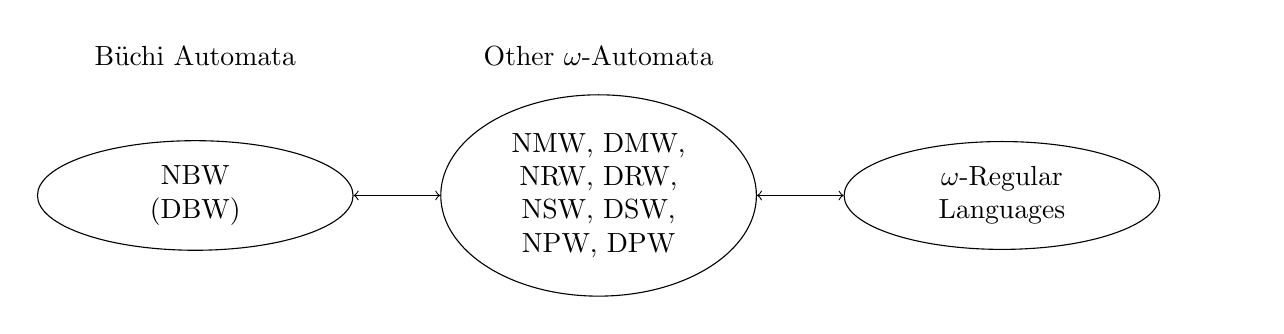
\begin{tikzpicture}[item/.style={ellipse,draw,text width=2.6cm,align=center}]
% \node[item] (left) {NBW\\(DBW)};
% \node [above=of left] {Büchi Automata};
% \node[item] (middle) [right=of left] {NMW, DMW,\\NRW, DRW,\\NSW, DSW,\\NPW, DPW};
% \node [above=of middle] {Other \om-Automata};
% \node[item] (right)  [right=of middle] {\om-Regular\\Languages};
\matrix[column sep=1.1cm,row sep=0.25cm]{
\node {Büchi Automata}; & \node {Other \om-Automata}; & & \\
\node[item] (left) {NBW\\(DBW)}; & \node[item] (middle) {NMW, DMW,\\NRW, DRW,\\NSW, DSW,\\NPW, DPW}; & \node[item] (right) {\om-Regular\\Languages}; &  \\
};
\path[<->] (left) edge (middle)
           (middle) edge (right);
\end{tikzpicture}
\caption{Non-deterministic Büchi automata (NBW) are expressively equivalent to Muller, Rabin, Streett, and parity automata (both deterministic and non-deterministic), and to the \om-regular languages. Deterministic Büchi automata (DBW) are less expressive than NBW.}
\label{equivalences}
\end{center}
\end{figure}


\subsection{Complementation of Büchi Automata}
\label{intro:complementation}
Büchi automata are closed under complementation. This result has been proved by Büchi himself when he introduced Büchi automata in~\cite{buchi1960decision}. Basically, this means that for every Büchi automata $A$, there exists another Büchi automaton $B$ that recognises the complement language of $A$, that is, $L(B) = \overline{L(A)}$.

It is interesting to see that this closure does not hold for the specific case of DBW. That means that while for every DBW a complement Büchi automaton does indeed exist, following from the above closure property for Büchi automata in general, this automaton is not necessarily a DBW. The complement of a DBW may be, and often is, as we will see, a NBW. This result is proved in~\cite{Thomas:1991} (p. 15).

The problem of Büchi complementation consists now in finding a procedure (usually called a construction) that takes as input any Büchi automaton $A$ and outputs another Büchi automaton $B$ with $L(B) = \overline{L(A)}$, as shown below.

\hbox to \hsize{\hfill{
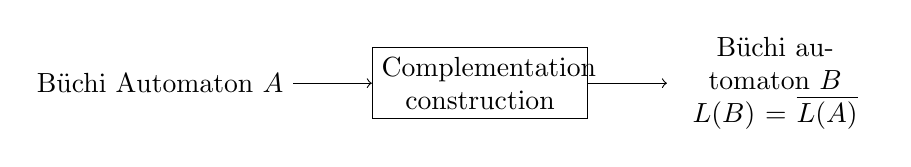
\begin{tikzpicture}[item/.style={rectangle,draw,text width=2.5cm,align=center}]
\node[] (left) {Büchi Automaton $A$};
\node[item] (middle) [right=of left] {Complementation construction};
\node[text width=2.5cm,align=center] (right)  [right=of middle] {Büchi automaton $B$\\$L(B) = \overline{L(A)}$}; 
\path[->] (left) edge (middle)
          (middle) edge (right);
\end{tikzpicture}}\hfill}

For complementation of automata in general, construction usually differ depending on whether the input automaton $A$ is deterministic or non-deterministic. Complementation of deterministic automata is often simpler and may sometimes even provide a solution for the complementation of the non-deterministic ones.

To illustrate this, we can briefly look at the complementation of the ordinary finite state automata on finite words (FA). FA are also closed under complementation~\cite{hopcroft2006automata} (p. 133). A DFA can be complemented by simply switching its accepting and non-accepting states~\cite{hopcroft2006automata} (p. 133). Now, since NFA and DFA are equivalent~\cite{hopcroft2006automata} (p. 60), a NFA can be complemented by converting it to an equivalent DFA first, and then complement this DFA. Thus, the complementation construction for DFA provides a solution for the complementation of NFA.

Returning to Büchi automata, the case is more complicated due to the inequivalence of NBW and DBW. The complementation of DBW is indeed ``easy'', as was the complementation of DFA. There is a construction, introduced in 1987 by Kurshan~\cite{Kurshan198759}, that can complement a DBW to a NBW in polynomial time. The size of the complement NBW is furthermore at most the double of the size of the input DBW.

If now for every NBW there would exist an equivalent DBW, an obvious solution to the general Büchi complementation problem would be to transform the input automaton to a DBW (if it is not already a DBW) and then apply Kurshan's construction to the DBW. However, as we have seen, this is not the case. There are NBW that cannot be turned into equivalent DBW.

Hence, for NBW, other ways of complementing them have to be found. In the next section we will review the most important of these ``other ways'' that have been proposed in the last 50 years since the introduction of Büchi automata. The Fribourg construction, that we present in Chapter~\ref{fribourg_construction}, is another alternative way of achievin this same aim.


\subsection{Complexity of Büchi Complementation}

Constructions for complementing NBW turned out to be very complex. Especially the blow-up in number of states from the input automaton to the output automaton is significant. For example, the original complementation construction proposed by Büchi~\cite{buchi1960decision} involved a doubly exponential blow-up. That is, if the input automaton has $n$ states, then for some constant $c$ the output automaton has, in the worst case, $c^{c^n}$ states~\cite{PrasadSistla1987217}. If we set $c$ to 2, then an input automaton with six states would result in a complement automaton with about 18 quintillion ($18 \times 10^{18}$) states.

Generally, state blow-up functions, like the $c^{c^n}$ above, mean the absolute worst cases. It is the maximum number of states a construction \emph{can} produce. For by far most input automata of size $n$ a construction will produce much fewer states. Nevertheless, worst case state blow-ups are an important (the most important?) performance measure for Büchi complementation constructions. A main goal in the development of new constructions is to bring this number down.

A question that arises is, how much this number can be brought down? Researchers have investigated this question by trying to establish so called lower bounds. A lower bound is a function for which it is proven that no state blow-up of any construction can be less than it. The first lower bound for Büchi complementation has been established by Michel in 1988 at $n!$~\cite{michel1988}. This means that the state blow-up of any Büchi complementation construction can never be less than $n!$.

There are other notations that are often used for state blow-ups. One has the form $(xn)^n$, where $x$ is a constant. Michel's bound of $n!$ would be about $(0.36n)^n$ in this case~\cite{2006_yan}. We will often use this notation, as it is convenient for comparisons. Another form has 2 as the base and a big-O term in the exponent. In this case, Michel's $n!$ would be $2^{O(n\,log\,n)}$~\cite{2006_yan}.

Michel's lower bound remained valid for almost two decades until in 2006 Yan showed a new lower bound of $(0.76n)^n$~\cite{2006_yan}. This does not mean that Michel was wrong with his lower bound, but just too reserved. The best possible blow-up of a construction can now be only $(0.76n)^n$ and not $(0.36n)^n$ as believed before. In 2009, Schewe proposed a construction with a blow-up of exactly $(0.76n)^n$ (modulo a polynomial factor)~\cite{schewe2009buchi}. He provided thus an upper bound that matches Yan's lower bound. The lower bound of $(0.76n)^n$ can thus not rise any further and seems to be definitve.

Maybe mention note on exponential complexity in \cite{1996_vardi} p. 8.


% \subsection{Complementation of Büchi Automata}
% It has been proved by Büchi himself that Büchi automata are closed under complementation~\cite{buchi1960decision}. That means that for every Büchi automaton, there exists another Büchi automaton accepting the complement language of the initial automaton.

% Let us denote by $L(A)$ the language recognised by Büchi automaton $A$. Then the complement language $\overline{L(A)}$ of $L(A)$ is $\overline{L(A)} = \Sigma^\omega \setminus L(A)$.

% \hbox to \hsize{\hfill{
% \begin{tikzpicture}[item/.style={rectangle,draw,text width=2.5cm}]
% \node[] (left) {$A$ with $L(A)$};
% \node[item] (middle) [right=of left] {Complementation algorithm};
% \node[] (right)  [right=of middle] {$B$ with $L(B) = \overline{L(A)}$}; 
% \path[->] (left) edge (middle)
%           (middle) edge (right);
% \end{tikzpicture}}\hfill}

% The problem of Büchi complementation can thus be summarised as follows. Given a Büchi automaton $A$, find a Büchi automaton $B$, such that $L(B) = \overline{L(A}$. For solving this problem we need an algorithm that takes $A$ as input and returns $B$ as output. 

% As a starting point, let us look at the complementation problem for normal finite state automata on finite words. Normal finite state automata recognise the regular languages and are also closed under complementation. For deterministic finite state automata, a possible complementation algorithm consists in simply inverting the accepting and non-accepting states of the automaton. Inuitively, every word that leaves the input automaton in an accepting state will leave the output automoaton in a non-accepting state, and vice versa. For the case of non-deterministic automata, one can take adavantage of the fact that every non-deterministic automata can be converted to an equivalent deterministic automaton. A standard algorithm for this conversion is the subset-construction, which is described in detail in [cite Hopcroft, Sec. 2.3.5]. The subset-construction basically takes all the subsets of states of the input automaton as states of the output automaton. A possible complementation algorithm for non-deterministic finite state automata consists thus in determinisation by the subset-construction and complementation by switching accepting and non-accepting states.

% Again, the cases of deterministic and non-deterministic automata are treated separately. For DBW, the method of switching accepting and non-accepting states does not work. Imagine for example that $\rho$ is the run of the word $x \in \Sigma^\omega$ of automaton $A$ (a DBW has exactly one run for every word of $\Sigma^\omega$). If $\textrm{inf}(\rho)$ contains both an accepting and a non-accepting state, then the switching of accepting and non-accepting states has no effect on the acceptance of $x$, as it is accepted in both cases. A working procedure for complementing DBW has been described by Kurshan [cite Kurshan, 1987]. Kurshan's construction is relatively easy and can be described in one sentence: make all states of the input automaton $A$ non-accepting, add another copy of $A$, remove all its accepting states and make the non-accepting states accepting, and finally add transitions from the states of the first copy of $A$ to the corresponding destination states in the second copy of $A$. The resulting automaton is an NBW $B$ that accepts the complement language of the input DBW $A$.

% In the case of finite-word automata, the complementation procedure for DFA provided a solution for the complementationn of NFA, because there is a translation from every NFA to an equivalent DFA. For Büchi automata this is however not the case. As mentioned above, there are NBW for which no equivalent DBW exists. We say that NBW can in general not be determinised.

\section{Run Analysis}
In a deterministic automaton every word has exactly one run. In a non-deterministic automaton, howevever, a given word may have multiple runs. The analysis of the different runs of a given word on an automaton plays an important role in the complementation of Büchi automata. There are several techniques for analysing the runs of a word that we present in this section.

\subsection{Run Trees}
The simplest of run analyis technique is the run tree. A run tree is a direct unfolding of all the possible runs of an automaton $A$ on a word $w$. Each vertex $v$ in the tree represents a state of $A$ that we denote by $\sigma(v)$. The descendants of a vetex $v$ on level $i$ are vertices representing the successor states of $\sigma(n)$ on the symbol $w(i+1)$ in $A$. In this way, every branch of the run tree originating in the root represents a possible run of automaton $A$ on word $w$.

Figure~\ref{run_tree} shows an example automaton $A$ and the first five levels of the run tree for the word $w = a^\omega$ (infinite repetitions of the symbol $a$). Each branch from the root to one of the leaves represents a possible way for reading the first four positions of $w$. On the right, as a label for all the edges on the corresponding level, is the symbol that causes the depicted transitions.

($A$ does not accept any word, it is empty. The only word it could accept is $a^\omega$ which it does not accept.)

We define by the width of a tree the maximum number of vertices occurring at any level~\cite{Muller199569}. Clearly, for \om-words the width of a run tree may become infinite, because there may be an infinite number of levels and each level may have more vertices than the previous one. 

\subsection{Failure of the Subset-Construction for Büchi Automata}
Run trees allow to conveniently reveal the cause why the subset construction does not work for determinising Büchi automata, which in turn motivates the basic idea of the next run analysis technique, split trees.

Applying the subset construction to the same NBW $A$ used in the previous example, we get the automaton $A^\prime$ shown in Figure~\ref{subset_construction_1}. Automaton $A^\prime$ is indeed a DBW but it accepts the word $a^\omega$ which $A$ does not accept. If we look at the run tree of $A$ on word $a^\omega$, the subset construction merges the individual states occuring at level $i$ of the tree to one single state $s_i$, which is accepting if at least one of its components is accepting. Equally, the individual transitions leading to and leaving from the individual components of $s_i$ are merged to a unified transition. The effect of this is that we lose all the information about these indiviudal transitions. This fact is depicted in Figure~\ref{subset_construction_2}. For the NFA acceptance condition this does not matter, but for NBW it is crucial because the acceptance condition depends on the history of specific runs. In the example in Figure~\ref{subset_construction_1}, a run $\rho$ of $A$ visiting the accepting state $q_1$ can never visit an accepting state anymore even though the unified run of which $\rho$ is part visits $q_1$ infinitely often. But the latter is achieved by infinitely many different runs each visiting $q_1$ just once.

It turns out that enough information about individual runs to ensure the Büchi acceptance condition could be kept, if accepting and non-accepting state are not mixed in the subset construction. Such a constructio has bee proposed in~\cite{UltesNitsche2007107}. Generally, the idea of treating accepting and non-accepting states separately is important in the run analyis of Büchi automata.





\subsection{Split Trees}
Split trees can be seen as run trees where the accepting and non-accepting descendants of a node $n$ are aggregated in two nodes. We will call the former the \emph{accepting child} and the latter the \emph{non-accepting child} of $n$. Thus in a split tree, every node has at most two descendants (if either the accepting or the non-accepting child is empty, it is not added to the tree), and the nodes represent sets of states rather than individual states. Figure~\ref{split_tree} shows the first five levels of the split tree of automaton $A$ on the word $a^\omega$.

The order in which the accepting and non-accepting child are 

The notion of split trees (and reduced split trees, see next section) has been introduced by Kähler and Wilke in 2008 for their slice-based complementation construction~\cite{2008_kaehler}, cf.~\cite{fogarty2013unifying}. However, the idea of separating accepting from non-accepting states has already been used earlier, for example in Muller and Schupp's determinisation-based complementation construction from 1995~\cite{Muller199569}. Formal definitions os split trees can be found in~\cite{2008_kaehler}\cite{fogarty2013unifying}.

\subsection{Reduced Split Trees}
The width of a split tree can still become infinitely large. A reduced split tree limits this width to a finite number with the restriction that on any level a given state may occur at most once. This is in effect the same as saying that if in a split tree there are multiple ways of going from the root to state $q$, then we keep only one of them. 


\subsection{Run DAGs}
A run DAG (DAG stands for directed acyclic graph) can be seen as a graph in matrix form with one column for every state of $A$ and one row for every position of word $w$. The edges are defined similarly than in run trees. Figure~\ref{run_dag} shows the run DAG of automaton $A$ on the word $w = a^\omega$. 

\section{Review of Büchi Complementation Constructions}
\label{review}
\subsection{Ramsey-Based Approaches}
\label{ramsey-based}
The method is called Ramsey-based because its correctness relies on a combinatorial result by Ramsey to obtain a periodic decomposition of the possible behaviors of a Büchi automaton on an infinite word~\cite{2012_breuers}.

\subsection{Determinisation-Based Approaches}
\label{det-based}
\subsection{Rank-Based Approaches}
\label{rank-based}
\subsection{Slice-Based Approaches}
\label{slice-based}

\section{Empirical Performance Investigations}

\chapter{The Fribourg Construction}
\label{fribourg_construction}
The Fribourg construction draws from several ideas: the subset construction, run analysis based on reduced split trees, and Kurshan's construction~\cite{Kurshan198759} for complementing DBW. Following the classification we used in Section~\ref{review}, it is a slice-based construction. Some of its formalisations are similar to the slice-based construction by Vardi and Wilke~\cite{vardi2007automata}, however, the Fribourg construction has been developed independently. Furthermore, as we will see in Chapter~\ref{results}, the empirical performance of Vardi and Wilke's construction and the Fribourg construction differ considerably, in favour of the latter.

Basically, the Fribourg construction proceeds in two stages. First it constructs the so-called upper part of the complement automaton, and then adds to it its so-called lower part. These terms stem from the fact that it is often convenient to draw the lower part below the previously drawn upper part. The partitioning in these two parts is inspired by Kurshan's complementation construction for DBW. The upper part of the Fribourg construction contains no accepting states and is intended to model the finite ``start phase'' of a run. At every state of the upper part, a run has the non-deterministic choice to either stay in the upper part or to move to the lower part. Once in the lower part, a run must stay there forever (or until it ends if it is discontinued). That is, the lower part models the infinite ``after-start phase'' of a run. The lower part now includes accepting states in a sophisticated way so that at least one run on word $w$ will be accepted if and only if all the runs of the input NBW on $w$ are rejected.

As it may be apparent from this short summary, the construction of the lower part is much more involved than the construction of the upper part.

\subsection{Construction of the Upper Part}
The construction of the upper part takes as input a NBW $A$ and outputs a deterministic automaton $B^\prime$ that will be the upper part of the final complement automaton $B$. The construction of $B^\prime$ is in its approach similar to the subset construction. One starts with a $B^\prime$-state representing the initial state of $A$ and then recursively determines and adds for each $B^\prime$-state one successor state per input symbol. The difference to the subset construction lies in the inner structure of the $B^\prime$-states. In the subset construction this would simply be a single set of $A$-states. In the subset-tuple construction, however, a $B^\prime$-state is a tuple of sets of $A$-states. A tuple is an ordered list, so differently phrased, a $B^\prime$-state consists of one or more sets of $A$-states where the order of these sets matters. As we will see, the $A$-states present in a $B^\prime$-state are the same that would result from the subset construction. But while in the subset construction all these states are thrown together in one set, in the subset-tuple construction they are split up in multiple sets where additionally the order of these sets is important. The subset-tuple construction can thus be seen as a modified subset construction that includes additional structure.

The structure of $B^\prime$-states is defined by ``level-clippings'' of reduced split trees, as we explain in a moment. But, talking about reduced split trees, we have to make a decision first. In Section~\ref{r_split_trees} we mentioned that reduced split trees come in equivalent left-to-right and right-to-left versions. The construction has to adopt one of these variants and stick to it. In this thesis we use the right-to-left version. The final complement automata look the same with either version except that the order of the tuples is reversed. Note that the optimisations described in Section~\ref{optmisations} is also based on this ordering and would need to be rephrased for the left-to-right version.

A new $B^\prime$-state $q$, successor on symbol $a$ of an already existing $B^\prime$-state $p$, now is created in the following way. The predecessor $p$ is regarded as a level of a reduced split tree by looking at its sets as the nodes on this level. Then, the next level for the given symbol $a$ is constructed as described in Section~\ref{r_split_tree}. This new level then directly defines $q$ by taking the nodes as the sets of $q$'s tuple and keeping their order. Figure~\ref{tree_to_slices} illustrates this with the example automaton $A$ that we already used before. If a state with a simlar tuple to the just created $q$ already exists in $B^\prime$, then just a transition from $p$ to this state is added (hence the loop in the third state of Figure~\ref{tree_to_slices}). The construction starts with a $B^\prime$-state containing only $A$'s initial state and ends when all states of $B^\prime$ have been processed for all input symbols. In Figure~\ref{tree_to_slices}, the construction is complete, thus the automaton shown at the right is the upper part of the complement of $A$.

If all the $A$-states of a $B^\prime$-state $p$ have no successors on an input symbol $a$, then $p$ will have no $a$-successor in $B^\prime$. This results in the upper part $B^\prime$ being incomplete at the end of the construction. In this case, it has to be made complete by adding a sink state. Furthermore, this sink state has to be accepting.

States of the subset-tuple construction are thus levels of reduced split trees. In the constructions of Varid and Wilke~\cite{vardi2007automata}, and Kähler and Wilke~\cite{2008_kaehler} states are called \emph{slices} of reduced split trees, hence the name slice-based approach.


\subsection{Construction of the Lower Part}
The construction of the lower part takes as input the upper part $B^\prime$ (and the initial automaton $A$) and outputs the final complement automaton $B$ with $L(B) = \c{L(A)}$. The construction of the lower part is basically an extension of the construction of the upper part that is applied to the states of the upper part. The extension consists therein that every set in the states of the lower part is assigned a \emph{colour}. These colours will be used to keep track of certain properties of runs of $B$ that finally allow to decide which states of the lower part of $B$ may be accepting. In this section we will first explain the mechanical construction of $B$ and give the intuition behind it afterwards.

There are three colours that sets of the lower part can have, let us call them 0, 1, and 2. The colour of a set says something about the history of the runs that reach this set. We have to clarify what we mean by run at this point. Conceptually, the subset-tuple construction unifies runs of the input automaton $A$. The construction conceptually includes two abstraction levels of this unification. Figure~\ref{runs} illustrates this. The figure shows three copies of two states of the upper part of the last section. The leftmost pair shows in dotted lines the runs of the original automaton $A$. These runs go from $A$-state to $A$-state, and are the ones that are unified by the construction. The middle part shows the conceptual unification of the $A$-runs to at most two outgoing branches per subset-tuple state, one for the accepting successors and one for the non-accepting successors. These runs go from state set to state set and correspond to the run analysis done with reduced split trees. The rightmost part finally shows the real run of the automaton excerpt. This is the run that is seen from the outside, when the inner structure of the states is now known. It unifies all the $A$-runs to one single run.

% Figure \label{runs}

In the following we will always refer to the notion of run in the middle of Figure~\ref{runs}. That is, the notion that directly corresponds to reduced split trees. This conceptual view unifies and simplifies the $A$-runs as much as possible, but still guards enough information for figuring out a correct acceptance behaviour of the final complement automaton $B$.

A run arriving at a set is thus a branch of a corresponding reduced split tree. It can be obtained by starting at the node corresponding to the set in question and following the edges upwards toward the root of the tree. A given set may occur in many reduced split trees, as there is a reduced split tree for every word of $A$'s alphabet. The set of runs arriving at a set are thus the corresponding branches of all the reduced split tree where the set occurs.

In the construction of the lower part, we are interested in the history of the runs back until the time when they left the upper part. The crucial information is whether this history of a run includes a so-called right-turn. The notion of right-turn can be understood figuratively. In a reduced split tree, a run can be thought of as having at any node $p$ the choice of either going to the accepting child of $p$ or to the non-accepting one. Since in the right-to-left version of reduced split trees accepting children are to the right of non-accepting children, the run literally ``turns right'' when going to the accepting child. Consequently, if a run has a right-turn in its history, then it has visited at least one accepting set since leaving the upper part. On the other hand, if a run has no right-turns in its history, then it has visited no accepting sets since leaving the upper part.

That leads us back to the colours that we use for labelling the sets of the lower part. The meaning of the colours 0, 1, and 2 is the following.
\begin{itemize}
\item 2: the run includes a right-turn in the lower part
\item 1: the run includes a right-turn in the lower part, but in the $B$-state where the run visited the accepting child, there was already another set with colour 2
\item 0: the run does not include right-turns in the lower part
\end{itemize}

The role of colour 0 and colour 2 should be clear from the above explanations. The role colour 1 is more subtle and we will explain it later in this section when we give the intuition behind the selection of the accepting states of $B$. For now, we will complete the description of how to construct the lower part and thereby the final complement automaton $B$.

As mentioned, constructing the states of the lower part is done in the same way as constructing the states of the upper part, with the difference that every set $s$ is assigned a colour. This colour depends on the colour of the predecessor set $s_{pred}$ of $s$ and on whether $s$ itself is an accepting or non-accepting set. Furthermore, there are different rules for the two cases where the $B$-state $p$ containing $s_{pred}$ contains one or more 2-coloured sets or does not contain any 2-coloured sets. Figure~\ref{colours} contains the complete rules for determining the colour of set $s$. Note that states of the upper part are treated as all their sets would have colour 0.

\begin{figure}
\begin{center}
\begin{tabular}{|C{3cm}|C{3cm}|C{3cm}|}
\hline
\raggedright $q_{pred}$: no 2-coloured sets & $s$ non-accepting & $s$ accepting \\
\hline
$c(s_{pred}) = 0$ & 0 & 2 \\
\hline
$c(s_{pred}) = 1$ & 2 & 2 \\
\hline
\end{tabular}
\vskip1em
\begin{tabular}{|C{3cm}|C{3cm}|C{3cm}|}
\hline
\raggedright $q_{pred}$: one or more 2-coloured sets   & $s$ non-accepting & $s$ accepting \\
\hline
$c(s_{pred}) = 0$ & 0 & 1 \\
\hline
$c(s_{pred}) = 1$ & 1 & 1 \\
\hline
$c(s_{pred}) = 2$ & 2 & 2 \\
\hline
\end{tabular}
\end{center}
\caption{Colour rules.}
\label{colours}
\end{figure}

The colour rules are in fact simple. The first rows in the two matrices in Figure~\ref{colours} treat the case where the run was still ``clean'' when it arrived at $s$'s predecessor $s_{pred}$. If now $s$ is the non-accepting child of $s_{pred}$, then the run stays clean and $s$ gets colour 0. But if $s$ is the accepting child, then the run just commits its first right-turn and gets dirty. Depending on whether there is another 2-coloured set in the state, $s$ gets either colour 1 or colour 2. The remaining rows in the matrices of Figure~\ref{colours} express the continuation of ``dirtiness''.




\section{Optimisations}
\label{optimisations}
\subsection{Removal of Non-Accepting States (R2C)}
\subsection{Merging of Adjacent Sets (M)}
\subsection{Reduction of 2-Coloured Sets (M2)}


\chapter{Performance Investigation of the Fribourg Construction}

\chapter{Results}
\label{results}

\chapter{Discussion}

\chapter{Conclusions}


\bibliographystyle{dwbibstyle}
\bibliography{../bibliography/buchi_complementation}


\end{document}